\documentclass[a4paper]{article}

\usepackage{amsmath}
\usepackage{amssymb,amsfonts}
\usepackage[catalan]{babel} % Language 
\usepackage{fontspec}
\usepackage[margin=2cm]{geometry}
\usepackage{graphicx}
\usepackage[makeroom]{cancel}
\usepackage{float}

\setlength{\parindent}{0pt}
\setlength{\parskip}{0.2cm}

\newcommand{\verteq}{\rotatebox{90}{$\,=$}}

\title{Tema 3: Mètodes de \emph{clustering}}

\begin{document}
	
\maketitle

\textbf{Objectiu}: El nostre objectiu és trobar agrupacions naturals de dades. Un grup o subgrup de dades és un \emph{cluster}

Les observacions que pertanyen al mateix \emph{cluster} s'assemblen entre elles

Les observacions que \textbf{no} pertanyen al mateix \emph{cluster} no s'assemblen tant

\textbf{\emph{Clustering:}}
\begin{itemize}
	\item el \textbf{procés} de trobar els \emph{clusters} presents en les dades
	\item el \textbf{resultat} del procés.
\end{itemize}

\begin{figure}[h!]
    \centering
    \begin{minipage}[t]{0.49\textwidth}
        \centering
        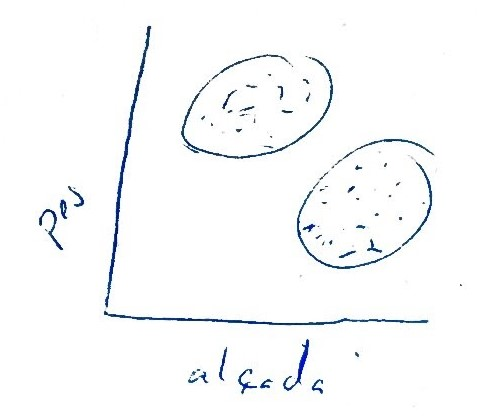
\includegraphics[width=\textwidth]{figura_1}
        \caption{Diversos grups}
    \end{minipage}
    \hfill
    \begin{minipage}[t]{0.49\textwidth}
        \centering
        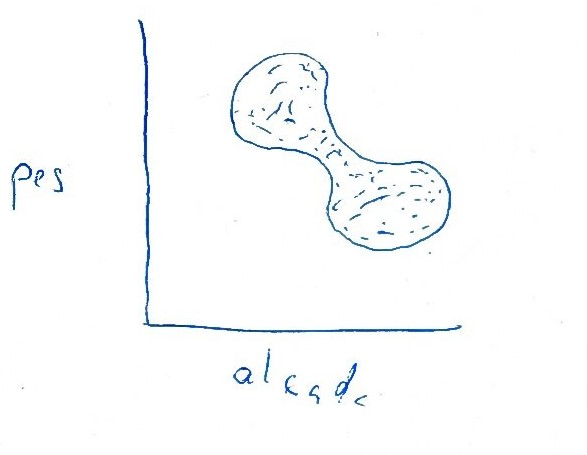
\includegraphics[width=\textwidth]{figura_2}
        \caption{Agrupar mitjançant clustering}
    \end{minipage}
\end{figure}

\section{Mètodes de \emph{clustering}}

Un tipus de mètode són els mètodes jeràrquics:
\begin{itemize}
	\item \textbf{divisius} es dediquen a separar les dades en dos grups recursivament fins que només queda un punt.
	\item \textbf{aglomeratius} es dediquen a agrupar les dades des d'un punt fins a obtenir el \emph{cluster} final.
\end{itemize}

\begin{figure}[H]
    \centering
    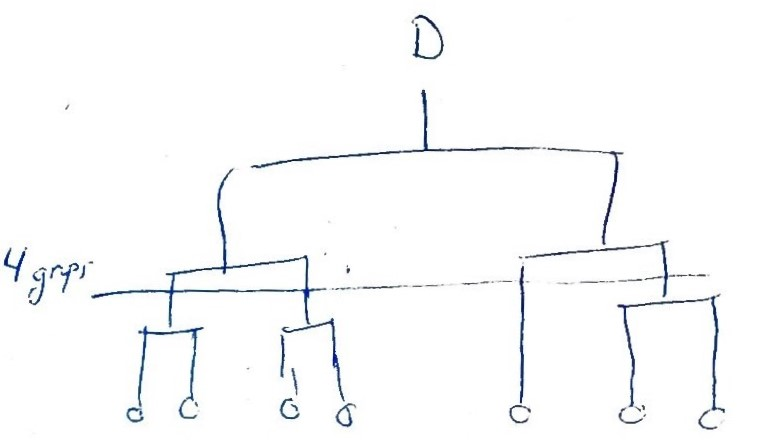
\includegraphics[width=0.5\textwidth]{figura_3}
    \caption{Mètodes jeràrquics}
\end{figure}

També hi ha els mètodes combinatoris. Hi ha un algoritme voraç amb una funció de qualitat.

Hi ha els algoritmes probabilístics. De quantes maneres es poden agrupar $N$ dades en $K$ \emph{clusters}?

$$ S(N, K) = \frac{1}{K!} \sum_{k=1}^K (-1)^{K-k} \begin{pmatrix}
K \\ k
\end{pmatrix} \text{, nº d'Stirling del 2n tipus} \implies S(19,4) \simeq 10^{10} $$

$$ \underbrace{B(N)}_{\text{nº de Bell}} \sum_{K=1}^{N} S(N,K) \implies \text{ ex.: } B(79) \simeq 3.89·10^85 $$

Així doncs hi ha diferents mètodes de \emph{clustering} per trobar els grups.

\section{Algorisme de $k$-means}

Tenim una mostra $\mathcal{D} = \{ x_1,..., x_N \} , x_i \in \mathbb{R}, 1 \le i \le N$. Fixa't $K$ externament, escollim un conjunt de $K$ \textbf{prototips}:

$$ \mathcal{P} = \{ \mu_1, ..., \mu_K \}, \mu \in \mathbb{R}^d $$

\begin{figure}[H]
    \centering
    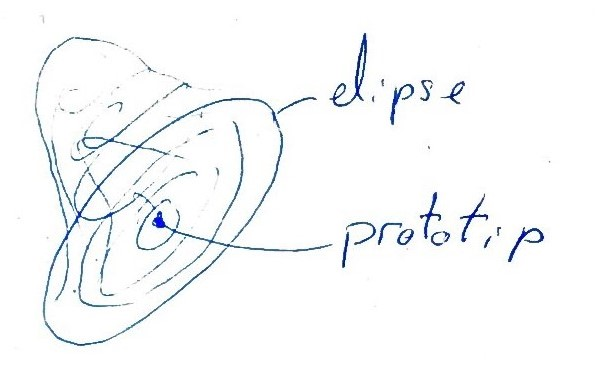
\includegraphics[width=0.5\textwidth]{figura_4}
    \caption{Anells d'agrupacions gaussianes}
\end{figure}

\begin{itemize}
	\item El nostre objectiu és trobar un conjunt de prototips $\mathcal{P}$ tal que les dades de $\mathcal{D}$ que estiguin assignades al \emph{cluster} $k$ es trobin més a prop de $\mu_k$ que de cap altre.
	\item Definim les variables indicadores:
	
	$$ r_{nk} =
	\begin{cases}
	1 & \text{si } k = argmin ||x_n - \mu_j||\ 1 \le j \le K \\ 0 & \text{en cas contrari}
	\end{cases}$$
	
	\item Definim un criteri de qualitat, a minimitzar, tenint en compte que minimitzar la distància al quadrat és el mateix que minimitzar la distància:
	
	$$ J(\mathcal{P}, \{r_{nk}\}) = \sum_{n=1}^N \sum_{k=1}^K r_{nk} ||x_n - \mu_k||^2 $$
	
	\begin{itemize}
		\item Si sapiguessim la solució per $\mathcal{P}$, com trobaríem la solució pells $\{r_{nk}\}$? Calculant les distàncies als $\mathcal{P}$.
		
		\item Si sapiguessim la solució per $\{r_{nk}\}$ com trobaríem la solució per $\mathcal{P}$? El prototip òptim és el centroide (la mitjana) de les dades assignades a cada \emph{cluster}.
	\end{itemize}
\end{itemize}

\subsection{Formalització}
\begin{itemize}
	\item Donat $\mathcal{P} = \{ \mu_1, ..., \mu_K \}$ recalcular els $\{r_{nk}\}$
	
	$$ r_{nk} =
	\begin{cases}
	1 & \text{si } k = argmin ||x_n - \mu_j||\ 1 \le j \le K \\ 0 & \text{en cas contrari}
	\end{cases}$$
	
	\item Recalcular $\mathcal{P}$ a partir dels $\{r_{nk}\}$
	
	\begin{itemize}
		\item $\frac{\partial J}{\partial \mu_k} = \sum_{n=1}^N r_{nk} \underbrace{\frac{\partial ||x_n - \mu_k||^2}{\partial \mu_k}}_{-2(x_n - \mu_k)} = 2\sum_{n=1}^N r_{nk} (\mu_k - x_n) = 0$
		
		$\sum_{n=1}^N r_{nk}\mu_k = \sum_{n=1}^N r_{nk}x_n \implies \mu_k\sum_{n=1}^N r_{nk} = \sum_{n=1}^N r_{nk}x_n \implies \boxed{\mu_k = \frac{\sum_{n=1}^N r_{nk}}{\sum_{n=1}^N r_{nk}}}$
		
		\item Tenint en compte que $\frac{\partial ||\vec{z}||^2}{\partial \vec{z}} = \begin{pmatrix}
		2z_1 \\ 2z_2 \\ \vdots \\ 2z_d
		\end{pmatrix} = 2\vec{z}$
	\end{itemize}
\end{itemize}

\subsection{Algorisme}

Inicialitzar $\mathcal{P}$

\textbf{Repetir}:
\begin{itemize}
	\item Re-calcular els $r_{nk}$ usant $\mathcal{P}$
	\item Re-calcular $\mathcal{P}$ usant els $r_{nk}$
\end{itemize}
\textbf{fins que} convergeixi

\textbf{retornar} $\mathcal{P},r_{nk}$


\subsection{Comentaris}

\begin{enumerate}
	\item $\Downarrow$ Cal una inicialització de $\mathcal{P}$, que és un problema en sí mateix
	\item $\Downarrow$ L'assignació de dades als \emph{clusters} $\{r_{nk}\}$ és \textbf{binària} per tant és difícil.
	\item $\Downarrow$ Cal un procediment extern de determinació de $K$.
\end{enumerate}

\section{Barreges de Gaussianes (Mixture of Gaussians)}

Determinació de \textbf{funcions de densitat de probabilitat (pdf)}. Tenim una mostra de dades  $\{x_1,...,x_n\}$ i.i.d (simple) generar una pdf $p(x)$. Això és impossible a no ser que reduïm les possibilitats.

El que farem serà agafar unes quantes gaussianes i comprovar quin percentatge de la solució final representen.

\begin{figure}[H]
    \centering
    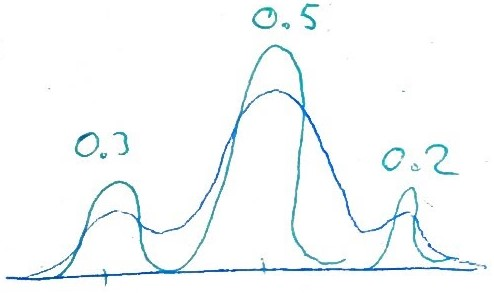
\includegraphics[width=0.5\textwidth]{figura_5}
    \caption{Barreja de Gaussianes}
\end{figure}

En dues dimensions es tenen unes dades podem trobar uns conjunts de gaussianes, es solaparan perquè les gaussianes tenen amplada infinit. Un cop trobades les ponderem i busquem la densitat final.

\begin{figure}[H]
    \centering
    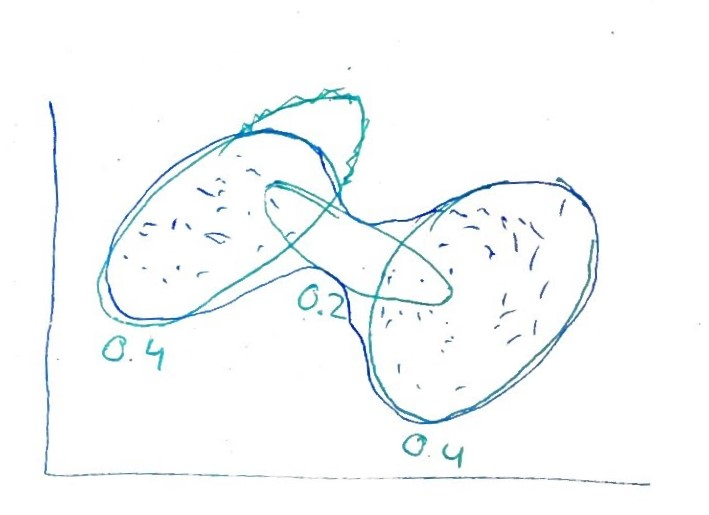
\includegraphics[width=0.5\textwidth]{figura_6}
    \caption{Diverses agrupacions Gaussianes}
\end{figure}

Una barreja de Gaussianes és una pdf de la forma:

$$ p(x) = \sum_{k=1}^K \underbrace{\pi_k}_{\text{Coeficients}}·\underbrace{N(x, \mu_k, \Sigma_k)}_{\text{Components de la barreja}}, 0 \le \pi_k \le 1, \sum_{k=1}^K \pi_k = 1$$

\begin{align*}
	\{\pi_k, \mu_k, \Sigma_k\} & \text{  desconegudes, paràmetres} \\
	K & \text{  desconegudea (hiper-paràmetre)}
\end{align*}

A vegades generalitzar el problema ajudar a trobar solucions que a simple vista no es poden veure per casos particulars. 

En principi la distribució $p$ només pertany de les variables $x$. Creem una nova variable aleatòria $z$ que ens ajuda a veure el problema de manera més general.

$$
p(\underbrace{x}_{x \in \mathbb{R}^d}) \rightarrow p(x,z) = p(x|z)·p(z)
$$

$$ 
z = 
\begin{pmatrix}
z1 \\ \vdots \\ z_K
\end{pmatrix} \text{Només una component de z és 1} 
$$

$$
z = 
\begin{pmatrix}
0 \\
0 \\
1 \\
0 \\
0
\end{pmatrix}
\rightarrow
\parbox{14em}{La $x$ associada a $z$ ha estat generada per la componen $k=3$ (amb probabilitat $\pi_3$)}
$$

S'interpreta com que ha estat la coponent $k$ la que ha generat X. Aquestes $z$ s'anomenen \textbf{variables aleatòries latents o ocultes}.

\begin{description}
	\item[Distribució marginal sobre z] $p(z_k = 1) = \pi_k$
	
	$p(z) = \prod_{k=1}^K {\pi_k}^{z_k}$
	
	\item[Distribució condicional] de $x$ respecte $z$
	
	$p(x|z_k = 1) = N(x, \mu_k, \Sigma_k)$
	
	\item[Distribució marginal sobre $x$] ara eliminem la $z$
	
	$p(x) = \sum_z p(x|z)p(z) = \sum_{k=1}^K \pi_k N(x, \mu_k, \Sigma_k)$
	
	\item[Distribució condicional] de $z$ respecte $x$
	
	$p(z_k = 1|x) = \frac{p(x|z_k = 1)p(z_k = 1)}{p(x)} = 
	\frac{N(x, \mu_k, \Sigma_k)·\pi_k}{\sum_{j=1}^K \pi_j · N(x, \mu_j, \Sigma_j)}$
	
	$\gamma_k(x) := p(z_k = 1 | x) \rightarrow \parbox{14em}{Probabilitat de que $x$ hagi estat generada per la component $k$ }$
	
	$\pi_k \rightarrow$ Prioritat a priori
	
	$p(z_k = 1 | x) \rightarrow$ Prioritat a posteriori
\end{description}

\subsection{Problema d'estimació de paràmetres: $\{\pi_k\}, \{ \mu_k \}, \{ \Sigma_k \}$ }

\subsubsection{Màxima versemblança}

$$ \{\pi_k\}, \{ \mu_k \}, \{ \Sigma_k \} = \theta $$

$$ 
\ell(\theta) = ln \mathcal{L}(\theta) = ln P(\mathcal{D}|\theta) =
ln \prod_{n=1}^N P(x_n | \{\pi_k, \mu_k, \Sigma_k \}) =
ln \prod_{n=1}^N \sum_{k=1}^K \pi_k N(x_n, \mu_k, \Sigma_k) = 
\sum_{n=1}^N ln\left(\sum_{k=1}^K \pi_k N\left(x_n, \mu_k, \Sigma_k \right) \right)
$$

$$
N(x, \mu, \Sigma) = \underbrace{|\Sigma|^{-\frac{1}{2}}·(2\pi)^{-\frac{d}{2}}}_C·exp\left( -\frac{1}{2}(x - \mu)^T \Sigma^{-1}(x-\mu) \right)
$$

\begin{flalign*}
	\textbullet &\frac{\partial \ell(\theta)}{\partial \mu_k} = \sum_{n=1}^N =
	\frac{1}{\sum_{j=1}^K \pi_j · N(x_n, \mu_j, \Sigma_j)}·\pi_k · \frac{\partial N(x_n, \mu_k, \Sigma_k}{\partial \mu_k} = 
	\sum_{n=1}^N 
	\underbrace{
		\frac{\pi_k·N(x_n, \mu_k, \Sigma_k)}{\sum_{j=1}^K \pi_j · N(x_n, \mu_j, \Sigma_j)}
	}_{\gamma_k(x_n)} \Sigma_k^{-1} (x_n - \mu_k) = &&\\
	&\sum_{n=1}^N \gamma_k (x_n) · \Sigma_k^{-1} (x_n - \mu_k) = 0 \implies \sum_{n=1}^N \gamma_k (x_n) · \Sigma_k^{-1} x_n = \sum_{n=1}^N \gamma_k(x_n) · \Sigma_k^{-1} \mu_k \implies \\
	&\cancel{\Sigma_k^{-1}} \left(\sum_{n=1}^N \gamma_k(x_n)·x_n \right) = \cancel{\Sigma_k^{-1}} \mu_k \left( \sigma_{n=1}^N \gamma_k(x_n) \right) \implies
	\boxed{\mu_k = \frac{\sum_{n=1}^N \gamma_k (x_n) · x_n}{\sum_{n=1}^N \gamma_k(x_n)}}
\end{flalign*}

\begin{flalign*}
	\textbullet \frac{\partial N(x, \mu, \Sigma}{\partial \mu} = 
	C·exp\left( -\frac{1}{2}(x - \mu)^T \Sigma^{-1}(x-\mu) \right) · \left(\cancel{-\frac{1}{2}}\right)·\underbrace{\frac{\partial \left\{ (x - \mu)^T \Sigma^{-1} (x - \mu) \right\} }{\partial \mu}}_{\cancel{-2}\Sigma^{-1}(x-\mu)} = 
	N(x,\mu,\Sigma)\Sigma^{-1}(x-\mu) &&
\end{flalign*}
\begin{flalign*}
	&\textbullet \frac{\partial z^T A z}{\partial z} = (A + A^T) z \underbrace{=}_{\parbox{3em}{\tiny Si A és simètrica}} 2Az &&
\end{flalign*}

\begin{flalign*}
	\textbullet\frac{\partial \ell(\theta)}{\partial \Sigma_k} = 0 \implies 
	\boxed{\Sigma_k = \frac{\sum_{n=1}^N \gamma_k(x_n) (x_n - \mu_k)(x_n - \mu_k)^T}{\sum_{n=1}^N \gamma_k (x_n)}}
	&&
\end{flalign*}

\begin{flalign*}
	\textbullet &\sum_{n=1}^K \pi_k = 1 \implies mcx\ \ell(\theta) + \lambda·\left( \sum_{k=1}^K \pi_k - 1 \right) \\
	& \frac{\partial \ell(\theta)}{\partial \pi_k} =
	\sum_{n=1}^N \frac{1}{\sum_{j=1}^K \pi_j·N(x_n,\mu_j, \Sigma_j)}·N(x_n,\mu_k,\Sigma_k) + \lambda = 0 \underset{\times\pi_k}{\implies} \underset{\forall k, 1 \le k \le K}{\sum_{n=1}^N \gamma_k(x_n) + \lambda \pi_k = 0} \implies
	\\
	& \sum_{k=1}^K \sum_{n=1}^N \gamma_k(x_n) + \lambda \underbrace{\sum_{k=1}^K \pi_k}_1 = 0 \implies \sum_{n=1}^N \underbrace{\sum_{k=1}^K \gamma_k(x_n)}_1 + \lambda = 0 \implies N + \lambda = 0 \implies \boxed{\lambda = -N} &&
\end{flalign*}

$$
\boxed{\pi_k = \frac{1}{N} \sum_{n=1}^N \gamma_k(x_n)}
$$

\subsubsection{Algorisme E-M Moos $(\mathcal{D},K)$}

Aquest algoritme serveix en general per maximitzar una funció de versemblança complexa.

\begin{itemize}
	\item Inicialitzar $ \{ \pi_k, \Sigma_k, \mu_k, 1 \le k \le K \} $
	\begin{itemize}
		\item $k-means(\mathcal{D},K) \circlearrowleft \rightarrow 
		\begin{cases}
			\mu_k \\
			\{ r_{nk} \} 
			\begin{cases}
				\Sigma_k \\
				\pi_k
			\end{cases}
		\end{cases}$
	\end{itemize}
	\item Repetir
	\begin{itemize}
		\item Calcular $\gamma_k(x_n), \forall k, \forall n \leftarrow$ calcular els \textbf{valors esperats} de les probabilitats a posteriori $\gamma_k (x_n)$
		\item Calcular les $ \{ \pi_k, \mu_k, \Sigma_k \},\ \forall k \leftarrow $ calcular per \textbf{maximització directa} (par M)
	\end{itemize}
\end{itemize}

\end{document}